\chapter{DevOps e code management}
\label{cap:devops}

\begin{inbreve}
DevOps unisce in un solo team lo sviluppo, il rilascio e il supporto del software, che un tempo erano affidati a team
separati. Il capitolo parte dai problemi dell'organizzazione tradizionale e definisce principi, benefici e cultura di
DevOps. Poi descrive le sue basi tecniche: il code management, l'automazione (continuous integration, delivery e
deployment, infrastructure as code) e la misura del processo e del prodotto. Si chiude con la cultura di ingegneria di
Spotify. Presuppone i capitoli~\ref{cap:agile}, \ref{cap:microservizi} e~\ref{cap:testing}.
\end{inbreve}

\section{Perché DevOps}
\label{sec:devops-perche}

\subsection{Team separati}

Tradizionalmente lo sviluppo, il rilascio e il supporto del software sono responsabilità di team separati
(\figrif{fig:devops-team}).
\begin{itemize}
  \item Il team di sviluppo passa la versione ``finale'' del software al team di rilascio.
  \item Il team di rilascio costruisce la versione da rilasciare, la collauda, prepara la documentazione del rilascio e
    rilascia il software ai clienti.
  \item Il team di supporto offre assistenza ai clienti.
\end{itemize}
Le modifiche al software le realizza il team di sviluppo, o un team di manutenzione separato.

\begin{figure}[ht]
\centering
\begin{tikzpicture}[b/.style={blocco, minimum width=2.4cm}, o/.style={draw, ellipse, font=\footnotesize, align=center, inner sep=1pt}]
\node[b] (d) at (0,0) {Development};
\node[b] (r) at (4.2,0) {Release};
\node[b] (s) at (8.4,0) {Support};
\node[o] (t) at (2.1,-1.6) {Tested software\\ready for release};
\node[o] (u) at (6.3,-1.6) {Deployed software\\ready for use};
\node[o] (p) at (4.2,1.6) {Problem and\\bug reports};
\draw[freccia] (d) -- (t);
\draw[freccia] (t) -- (r);
\draw[freccia] (r) -- (u);
\draw[freccia] (u) -- (s);
\draw[freccia] (s.north) |- (p.east);
\draw[freccia] (p.west) -| (d.north);
\end{tikzpicture}
\caption{Sviluppo, rilascio e supporto affidati a tre team. Ogni team passa il proprio prodotto al successivo; le
segnalazioni di problemi e bug raccolte dal supporto tornano allo sviluppo.}
\label{fig:devops-team}
\end{figure}

Questa organizzazione ha dei problemi.
\begin{itemize}
  \item Ci sono ritardi di comunicazione tra i team.
  \item I team usano strumenti diversi e hanno competenze diverse. Spesso non capiscono i problemi degli altri.
  \item Servono giorni per correggere bug urgenti o vulnerabilità di sicurezza.
\end{itemize}
Il risultato è una risposta lenta alle esigenze del business. Servono settimane per distribuire nell'ambiente di
produzione. Il codice nuovo va adattato a fatica per entrare nell'ambiente di produzione, e le distribuzioni vanno
pianificate.

\subsection{L'approccio DevOps}
\label{sec:devops-approccio}

Tre fattori hanno reso possibile un cambiamento.
\begin{enumerate}
  \item L'ingegneria del software agile (capitolo~\ref{cap:agile}) ha ridotto i tempi di sviluppo. Il processo di
    rilascio tradizionale è diventato il collo di bottiglia.
  \item Amazon ha riprogettato il proprio software in (micro)servizi e ha assegnato allo stesso team sia lo sviluppo
    sia il supporto di un servizio.
  \item È diventato possibile rilasciare il software come servizio (SaaS) su cloud pubblici e privati
    (capitolo~\ref{cap:cloud}).
\end{enumerate}

\begin{definizione}[DevOps]
DevOps (\emph{Development} + \emph{Operations}) integra sviluppo, distribuzione e supporto in un
\textbf{unico team}.
\end{definizione}

La definizione estende quella data per i microservizi (\rif{sec:micro-distribuzione}). Con DevOps:
\begin{itemize}
  \item i team di sviluppo e di operations sono integrati, per migliorare collaborazione e produttività;
  \item si automatizzano i test, i flussi di lavoro e l'infrastruttura;
  \item si misurano di continuo le prestazioni dell'applicazione;
  \item l'ambiente di sviluppo è uguale all'ambiente di produzione;
  \item i rilasci sono più frequenti;
  \item la risposta alle esigenze del business è più veloce.
\end{itemize}
Serve una nuova mentalità e servono nuovi strumenti:
\begin{itemize}
  \item gestione dei sorgenti (\ingl{source control}, per esempio GitHub, \rif{sec:devops-codice});
  \item build e test continui del codice (per esempio Jenkins, Travis, \rif{sec:devops-ci});
  \item gestione della configurazione (per esempio Puppet, Chef, SaltStack, Ansible, \rif{sec:devops-iac});
  \item monitoraggio delle prestazioni dell'applicazione (\ingl{application performance monitoring}, APM; per esempio
    New Relic, Pingdom Server Monitor, \rif{sec:devops-misura}).
\end{itemize}

\subsubsection{Le radici di DevOps}
DevOps mette insieme idee nate altrove:
\begin{itemize}
  \item il manifesto per lo sviluppo agile (\rif{sec:agile-manifesto});
  \item le architetture a microservizi (capitolo~\ref{cap:microservizi});
  \item il \emph{Lean Software Development}, con sette principi:
    \begin{enumerate}
      \item eliminare gli sprechi;
      \item amplificare l'apprendimento;
      \item decidere il più tardi possibile;
      \item consegnare il più presto possibile;
      \item dare responsabilità al team;
      \item costruire l'integrità dentro il prodotto;
      \item vedere l'insieme;
    \end{enumerate}
  \item il \emph{Toyota Production System}, con due concetti: \emph{kaizen}, il miglioramento continuo, e
    \emph{jidoka}, ``fermare la produzione perché la produzione non debba mai fermarsi''.
\end{itemize}

\subsection{Principi, benefici e cultura}
\label{sec:devops-principi}

\begin{definizione}[Principi di DevOps]
\begin{description}[leftmargin=0pt, style=unboxed]
  \item[Everyone is responsible for everything.] Tutti i membri del team sono responsabili insieme dello sviluppo, della
    consegna e del supporto del software.
  \item[Everything that can be automated should be automated.] Tutte (o quasi) le attività di test, distribuzione e
    supporto vanno automatizzate.
  \item[Measure first, change later.] DevOps è guidato dalla misura: si raccolgono dati sul sistema e sul suo
    funzionamento, e si cambia in base a quei dati.
\end{description}
\end{definizione}

I benefici sono quattro.
\begin{description}[leftmargin=0pt, style=unboxed]
  \item[Distribuzione più veloce.] I ritardi di comunicazione tra persone si riducono drasticamente, quindi si va in
    produzione più in fretta.
  \item[Rischio ridotto.] Ogni rilascio aggiunge un piccolo incremento di funzionalità. C'è meno probabilità di
    interazioni tra feature e di guasti o interruzioni del sistema.
  \item[Riparazione più veloce.] Non bisogna scoprire quale team è responsabile del problema e aspettare che lo
    risolva.
  \item[Team più produttivi.] I team DevOps sono più produttivi dei team che si occupano di attività separate.
\end{description}

Creare un team DevOps significa mettere insieme competenze diverse:
\begin{itemize}
  \item ingegneria del software;
  \item progettazione dell'esperienza utente (UX design);
  \item ingegneria della sicurezza;
  \item ingegneria dell'infrastruttura;
  \item interazione con i clienti.
\end{itemize}
Un team DevOps che funziona ha una \textbf{cultura di rispetto reciproco e di condivisione}. Gli sviluppatori
dovrebbero dare supporto ai servizi software che hanno sviluppato.

\section{Code management}
\label{sec:devops-codice}

\begin{definizione}[Code management]
Il \termine{code management} gestisce l'evoluzione del codebase. Ha due obiettivi:
\begin{itemize}
  \item memorizzare e recuperare le versioni dei componenti e dei sistemi interi;
  \item permettere agli sviluppatori di lavorare in parallelo senza interferire e di integrare il proprio lavoro.
\end{itemize}
\end{definizione}

Le funzionalità principali di un sistema di code management (per esempio Git) sono cinque.
\begin{itemize}
  \item Trasferire il codice dal filesystem dello sviluppatore al sistema e viceversa.
  \item Memorizzare e recuperare le versioni: i file non sono mai sovrascritti.
  \item \ingl{Branching} e \ingl{merging}: rami di sviluppo separati per il lavoro in parallelo, poi fusi.
  \item Informazioni sulle versioni e storia delle modifiche.
  \item Supporto ai progetti: tutti i file di un progetto si possono prelevare (\ingl{check out}) insieme.
\end{itemize}

Il code management è la \textbf{base dell'automazione DevOps} (CI/CD, infrastructure as code) e della misura
(\figrif{fig:devops-codice}).

\begin{figure}[ht]
\centering
\begin{tikzpicture}[s/.style={draw, rounded corners=3pt, fill=white, font=\footnotesize, align=center, minimum height=0.8cm}]
\draw[fill=grigiochiaro] (0,3.0) rectangle (9.6,4.6);
\node[font=\footnotesize\bfseries] at (4.8,4.35) {DevOps automation};
\node[s, minimum width=2.0cm] at (1.2,3.55) {Continuous\\integration};
\node[s, minimum width=2.0cm] at (3.6,3.55) {Continuous\\deployment};
\node[s, minimum width=2.0cm] at (6.0,3.55) {Continuous\\delivery};
\node[s, minimum width=2.0cm] at (8.4,3.55) {Infrastructure\\as code};
\draw[fill=grigiochiaro] (0,0) rectangle (9.6,2.4);
\node[font=\footnotesize\bfseries] at (4.8,2.15) {Code management system};
\node[font=\scriptsize] at (4.8,1.8) {Branching and merging};
\node[s, minimum width=3.6cm] at (4.8,1.05) {Code repository};
\node[font=\scriptsize, align=center] at (1.3,1.05) {Recover version\\information};
\node[font=\scriptsize, align=center] at (8.3,1.05) {Save and retrieve\\versions};
\node[font=\scriptsize] at (4.8,0.25) {Transfer code to/from developer's filestore};
\draw[fill=grigiochiaro] (0,-2.2) rectangle (9.6,-0.6);
\node[font=\footnotesize\bfseries] at (4.8,-0.85) {DevOps measurement};
\node[s, minimum width=2.2cm] at (2.0,-1.6) {Data collection};
\node[s, minimum width=2.2cm] at (4.8,-1.6) {Data analysis};
\node[s, minimum width=2.2cm] at (7.6,-1.6) {Report generation};
\draw[->, very thick, blu] (2.0,2.45) -- (2.0,2.95);
\draw[->, very thick, blu] (7.6,2.95) -- (7.6,2.45);
\draw[->, very thick, blu] (2.0,-0.55) -- (2.0,-0.05);
\draw[->, very thick, blu] (7.6,-0.05) -- (7.6,-0.55);
\end{tikzpicture}
\caption{Il sistema di code management al centro di DevOps. Sopra di esso lavorano gli strumenti di automazione, sotto
quelli di misura; entrambi leggono dal repository e vi scrivono (frecce).}
\label{fig:devops-codice}
\end{figure}

\section{DevOps automation}
\label{sec:devops-automazione}

Il principio ``tutto ciò che si può automatizzare va automatizzato'' si realizza con quattro pratiche.

\begin{definizione}[Le quattro pratiche di automazione]
\begin{description}[leftmargin=0pt, style=unboxed]
  \item[Continuous integration.] Ogni volta che uno sviluppatore fa il commit di una modifica sul ramo principale
    (\ingl{master branch}) del progetto, si costruisce e si collauda una versione eseguibile del sistema.
  \item[Continuous delivery.] Il software eseguibile è collaudato in un ambiente che simula l'ambiente operativo del
    prodotto.
  \item[Continuous deployment.] Una nuova versione del sistema è resa disponibile agli utenti ogni volta che si fa una
    modifica al ramo principale del software.
  \item[Infrastructure as code.] Modelli leggibili dalla macchina dell'infrastruttura su cui gira il prodotto (rete,
    server, router, ecc.) sono usati da strumenti di gestione della configurazione per costruire la piattaforma di
    esecuzione del software. Il software da installare, come compilatori, librerie e DBMS, fa parte del modello
    dell'infrastruttura.
\end{description}
\end{definizione}

\subsection{Continuous integration}
\label{sec:devops-ci}

Integrare il sistema (\ingl{system building}) è molto più che compilare. Bisogna:
\begin{itemize}
  \item installare il software del database e predisporre il database con lo schema giusto;
  \item caricare nel database i dati di test;
  \item compilare i file che compongono il prodotto;
  \item collegare il codice compilato con le librerie e gli altri componenti usati;
  \item controllare che i servizi esterni usati siano operativi;
  \item spostare i file di configurazione nelle posizioni giuste, cancellando quelli vecchi;
  \item eseguire i system test per controllare che l'integrazione sia riuscita.
\end{itemize}
Se il sistema si integra di rado, i problemi sono difficili da isolare e correggerli rallenta lo sviluppo. Per questo
si usa la continuous integration.

\begin{definizione}[Continuous integration]
Con la \termine{continuous integration} (CI) si crea e si collauda una versione integrata del sistema ogni volta che
una modifica è inviata (\ingl{push}) al repository condiviso del codice. Al termine del push il repository manda un
messaggio a un \termine{integration server}, che costruisce una nuova versione del prodotto (\figrif{fig:devops-ci}).
\end{definizione}

\begin{figure}[ht]
\centering
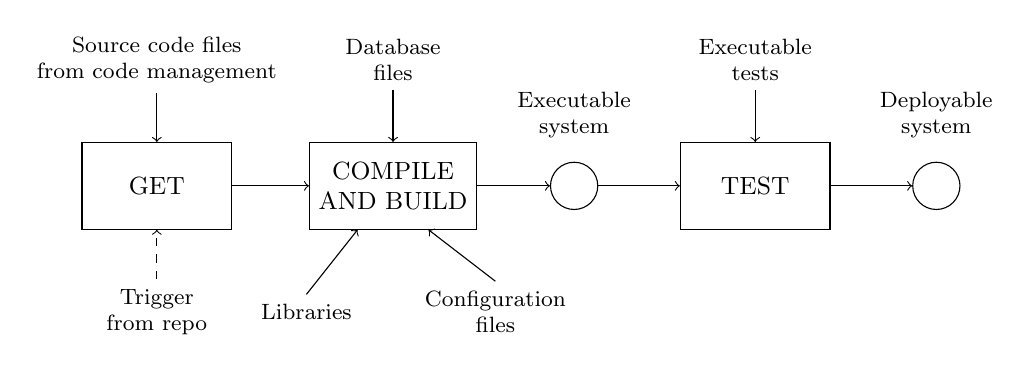
\begin{tikzpicture}[b/.style={draw, minimum width=1.9cm, minimum height=1.1cm, font=\small, align=center}]
\node[b] (g) at (0,0) {GET};
\node[b] (c) at (3.0,0) {COMPILE\\AND BUILD};
\node[draw, circle, minimum size=0.6cm] (e) at (5.3,0) {};
\node[b] (t) at (7.6,0) {TEST};
\node[draw, circle, minimum size=0.6cm] (d) at (9.9,0) {};
\draw[->] (g) -- (c);
\draw[->] (c) -- (e);
\draw[->] (e) -- (t);
\draw[->] (t) -- (d);
\node[font=\footnotesize, align=center] (src) at (0,1.6) {Source code files\\from code management};
\node[font=\footnotesize, align=center] (dbf) at (3.0,1.6) {Database\\files};
\node[font=\footnotesize, align=center] (et) at (7.6,1.6) {Executable\\tests};
\node[font=\footnotesize, align=center] at (5.3,0.9) {Executable\\system};
\node[font=\footnotesize, align=center] at (9.9,0.9) {Deployable\\system};
\node[font=\footnotesize, align=center] (lib) at (1.9,-1.6) {Libraries};
\node[font=\footnotesize, align=center] (cf) at (4.3,-1.6) {Configuration\\files};
\node[font=\footnotesize, align=center] (tr) at (0,-1.6) {Trigger\\from repo};
\draw[->] (src) -- (g);
\draw[->] (dbf) -- (c);
\draw[->] (et) -- (t);
\draw[->] (lib.north) -- ([xshift=-0.45cm]c.south);
\draw[->] (cf.north) -- ([xshift=0.45cm]c.south);
\draw[->, dashed] (tr) -- (g);
\end{tikzpicture}
\caption{Continuous integration. Il push sul repository fa partire l'integrazione (freccia tratteggiata). Si prelevano
i sorgenti, si compila e si costruisce il sistema con file del database, librerie e file di configurazione, si
eseguono i test eseguibili. Se riescono, il sistema è pronto per essere distribuito.}
\label{fig:devops-ci}
\end{figure}

\subsubsection{Non ``rompere la build''}
Chi invia codice che fa fallire l'integrazione ``rompe la build'' (\ingl{break the build}) e blocca il lavoro di tutti.
Per evitarlo si integra \textbf{due volte} (\ingl{integrate twice}, \figrif{fig:devops-due-volte}):
\begin{enumerate}
  \item si integra e si collauda sul proprio computer;
  \item si invia il codice al repository del progetto, che fa partire l'integration server.
\end{enumerate}

\begin{figure}[ht]
\centering
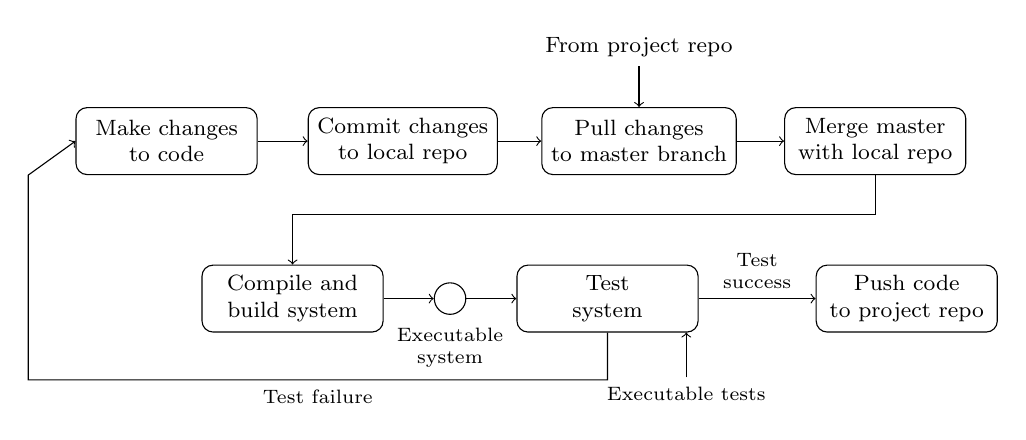
\begin{tikzpicture}[b/.style={draw, rounded corners=4pt, font=\footnotesize, align=center, minimum width=2.3cm, minimum height=0.85cm}]
\node[b] (a) at (0,0) {Make changes\\to code};
\node[b] (b) at (3.0,0) {Commit changes\\to local repo};
\node[b] (c) at (6.0,0) {Pull changes\\to master branch};
\node[b] (d) at (9.0,0) {Merge master\\with local repo};
\node[b] (e) at (1.6,-2.0) {Compile and\\build system};
\node[draw, circle, minimum size=0.4cm] (x) at (3.6,-2.0) {};
\node[b] (f) at (5.6,-2.0) {Test\\system};
\node[b] (g) at (9.4,-2.0) {Push code\\to project repo};
\node[font=\footnotesize] (fr) at (6.0,1.2) {From project repo};
\draw[->] (a) -- (b);
\draw[->] (b) -- (c);
\draw[->] (c) -- (d);
\draw[->] (fr) -- (c);
\draw[->] (d.south) -- ++(0,-0.5) -| (e.north);
\draw[->] (e) -- (x);
\draw[->] (x) -- (f);
\node[font=\scriptsize, anchor=north, align=center] at (3.6,-2.25) {Executable\\system};
\draw[->] (f) -- node[above, font=\scriptsize, align=center] {Test\\success} (g);
\draw[->] (f.south) -- ++(0,-0.6) -| node[pos=0.25, below, font=\scriptsize] {Test failure} ([xshift=-0.6cm]a.south west) -- (a.west);
\node[font=\scriptsize, anchor=north] at (6.6,-3.0) {Executable tests};
\draw[->] (6.6,-3.0) -- (6.6,-2.43);
\end{tikzpicture}
\caption{Integrare due volte. Lo sviluppatore fa il commit in locale, preleva le modifiche degli altri dal ramo
principale e le fonde con le proprie. Poi compila e collauda sul proprio computer: se i test falliscono torna a
modificare il codice, se riescono invia il codice al repository del progetto.}
\label{fig:devops-due-volte}
\end{figure}

\subsubsection{Vantaggi}
\begin{description}[leftmargin=0pt, style=unboxed]
  \item[Bug trovati e corretti più in fretta.] Se si fa una piccola modifica e un test di sistema fallisce, il problema
    sta quasi certamente nel codice appena inviato.
  \item[Un sistema funzionante è sempre disponibile per tutto il team.] Serve a provare idee e a mostrare il sistema
    ai dirigenti e ai clienti.
  \item[Cultura della qualità nel team.] Nessuno vuole lo stigma di aver rotto la build. Ognuno controlla con cura il
    proprio lavoro prima di inviarlo al repository del progetto.
\end{description}

\subsubsection{Build incrementale}
Gli strumenti di integrazione ripetono un'azione solo se i file da cui dipende sono cambiati
(\figrif{fig:devops-incrementale}).
\begin{itemize}
  \item Alla prima integrazione si compilano tutti i file sorgente e tutti i file dei test eseguibili.
  \item Nelle integrazioni successive si creano i file oggetto solo per i test e i sorgenti modificati.
\end{itemize}
Per sapere se un file è cambiato si confrontano le \emph{date di modifica} (\ingl{timestamp}):
\begin{itemize}
  \item data(codice compilato) $>$ data(codice sorgente) $\to$ non si fa nulla;
  \item data(codice compilato) $<$ data(codice sorgente) $\to$ si ricompila;
  \item data(codice compilato) $<$ data(definizione di classe) $\to$ si ricompila.
\end{itemize}

\begin{figure}[ht]
\centering
\begin{tikzpicture}[o/.style={draw, ellipse, font=\scriptsize, align=center, inner sep=1pt, minimum width=2.0cm}]
% sinistra
\node[o] (ps) at (0,2.6) {Program source\\code files};
\node[o] (ts) at (2.6,2.6) {Test source\\code files};
\node[o] (po) at (0,1.2) {Program object\\code files};
\node[o] (to) at (2.6,1.2) {Test object\\code files};
\node[blocco, font=\scriptsize] (te) at (1.3,-0.2) {Test execution};
\draw[->] (po) -- (ps);
\draw[->] (to) -- (ts);
\draw[->] (te) -- (po);
\draw[->] (te) -- (to);
% destra
\node[o, minimum width=1.2cm] (l1) at (6.0,2.6) {Lib 1};
\node[o, minimum width=1.2cm] (l2) at (7.6,2.6) {Lib 2};
\node[o] (cd) at (9.6,2.6) {Classdef\\(compiled)};
\node[o] (ms) at (7.6,1.2) {Mycode\\(source)};
\node[o] (mc) at (7.6,-0.2) {Mycode\\(compiled)};
\draw[->] (ms) -- (l1);
\draw[->] (ms) -- (l2);
\draw[->] (ms) -- (cd);
\draw[->] (mc) -- (ms);
\end{tikzpicture}
\caption{Dipendenze in una build incrementale. Una freccia da A a B significa che A dipende da B. A sinistra
l'esecuzione dei test dipende dai file oggetto, che dipendono dai sorgenti. A destra il codice compilato dipende dal
sorgente, che dipende da due librerie e da una definizione di classe compilata. Se B è più recente di A, A va
ricostruito.}
\label{fig:devops-incrementale}
\end{figure}

\subsubsection{Strumenti}
\begin{itemize}
  \item Strumenti di build del sistema: Unix \texttt{make} (il più vecchio), Ant e Maven (Java), Rake (Ruby).
  \item Strumenti di continuous integration: Jenkins (open source), Travis, Bamboo, GitHub Actions.
\end{itemize}

\subsection{Continuous delivery e continuous deployment}
\label{sec:devops-cd}

La continuous integration crea una versione eseguibile del sistema costruendolo e collaudandolo sul computer dello
sviluppatore o sull'integration server del progetto. L'ambiente di produzione reale però sarà diverso dall'ambiente di
sviluppo.
\begin{itemize}
  \item Il server di produzione può avere un'organizzazione del filesystem, permessi di accesso e applicazioni
    installate diversi.
  \item Possono comparire bug nuovi.
\end{itemize}

La \termine{continuous delivery} assicura che il sistema modificato sia pronto per essere consegnato ai clienti. Lo fa
con:
\begin{itemize}
  \item feature test nell'ambiente di produzione, per essere certi che l'ambiente non causi guasti del sistema;
  \item load test, per controllare come si comporta il software quando il numero di utenti cresce.
\end{itemize}
I container (capitolo~\ref{cap:container}) sono il modo più semplice per creare una replica dell'ambiente di
produzione.

\figrif{fig:devops-cd} mostra le due fasi.
\begin{description}[leftmargin=0pt, style=unboxed]
  \item[Per consegnare (deliver).] Dopo i primi test di integrazione si configura un ambiente di test a tappe
    (\ingl{staged}) che replica l'ambiente di produzione. Lì si eseguono gli acceptance test del sistema: funzionalità,
    carico, prestazioni.
  \item[Per distribuire (deploy).] Software e dati sono trasferiti sui server di produzione. Si smette di accettare
    nuove richieste di servizio e si lascia che la versione vecchia completi le transazioni in corso. Poi si passa alla
    nuova versione del sistema e si riprende l'elaborazione.
\end{description}

\begin{figure}[ht]
\centering
\begin{tikzpicture}[b/.style={draw, font=\footnotesize, align=center, minimum width=2.2cm, minimum height=0.85cm}]
\draw[fill=grigiochiaro] (-0.3,-0.75) rectangle (8.1,0.75);
\node[b, fill=white] (a) at (1.0,0) {Configure\\test server};
\node[b, fill=white] (b) at (3.9,0) {Install system\\on test server};
\node[b, fill=white] (c) at (6.8,0) {Run acceptance\\tests};
\draw[->] (a) -- (b);
\draw[->] (b) -- (c);
\node[font=\footnotesize, anchor=north west] at (-0.3,-0.8) {Continuous delivery};
\foreach \x/\t in {1.0/Required\\software, 3.9/Tested\\system, 6.8/Test\\set} {
  \node[draw, circle, minimum size=0.4cm] (k) at (\x,1.5) {};
  \node[font=\scriptsize, align=right, anchor=east] at (\x-0.3,1.5) {\t};
  \draw[->] (k) -- (\x,0.75);
}
\draw[fill=grigiochiaro] (-0.3,-3.3) rectangle (5.6,-1.8);
\node[b, fill=white] (d) at (1.2,-2.55) {Install software on\\production servers};
\node[b, fill=white] (e) at (4.2,-2.55) {Switch operation\\to new software};
\draw[->] (d) -- (e);
\node[font=\footnotesize, anchor=north west] at (-0.3,-3.35) {Continuous deployment};
\draw[->] (c.south) -- ++(0,-1.2) -| node[pos=0.25, above, font=\scriptsize] {All tests pass} (d.north);
\end{tikzpicture}
\caption{Continuous delivery e deployment. Nella delivery si configura un server di test che replica la produzione, vi
si installa il sistema già collaudato e si eseguono gli acceptance test. Se passano tutti, nel deployment si installa il
software sui server di produzione e si passa alla nuova versione.}
\label{fig:devops-cd}
\end{figure}

Un esempio di pipeline completa, per un microservizio, è in \figrif{fig:micro-pipeline}.

\subsubsection{Benefici della continuous deployment}
\begin{description}[leftmargin=0pt, style=unboxed]
  \item[Costi ridotti.] La pipeline di distribuzione è completamente automatica.
  \item[Problemi risolti più in fretta.] Se c'è un problema, probabilmente tocca solo una piccola parte del sistema e
    la sua origine è evidente.
  \item[Feedback dei clienti più veloce.] Si possono distribuire nuove feature appena sono pronte per i clienti. Il
    feedback degli utenti serve a trovare miglioramenti.
  \item[A/B testing.] Se si hanno molti clienti e diversi server:
    \begin{itemize}
      \item si distribuisce la nuova versione del software solo su alcuni server;
      \item il load balancer dirotta una parte dei clienti verso la nuova versione;
      \item si misura e si valuta come sono usate le nuove feature.
    \end{itemize}
\end{description}
La continuous deployment è praticabile solo per i sistemi basati sul cloud.

\subsubsection{Perché non distribuire ogni singola modifica?}
Ci sono ragioni di business per non distribuire ai clienti ogni modifica del software.
\begin{enumerate}
  \item Ci sono feature incomplete che si potrebbero distribuire, ma non si vuole mostrarle ai concorrenti finché non
    sono complete.
  \item I clienti possono irritarsi se il software cambia di continuo, soprattutto quando cambia l'interfaccia utente.
  \item Si vogliono sincronizzare i rilasci con cicli di business noti, per esempio l'inizio dell'anno accademico per
    il mercato dell'istruzione.
\end{enumerate}

\subsubsection{Strumenti}
Gli strumenti di CI come Jenkins e Travis si usano anche per la continuous delivery e il deployment. Si integrano con gli
strumenti di gestione della configurazione dell'infrastruttura, come Chef, Puppet e Ansible, per distribuire il
software. Per il software basato sul cloud spesso è più semplice usare i container insieme agli strumenti di CI che
usare software di gestione della configurazione dell'infrastruttura.

\subsection{Infrastructure as code}
\label{sec:devops-iac}

Gestire a mano un'infrastruttura di decine o centinaia di server è costoso e soggetto a errori.
\begin{itemize}
  \item Ci sono molti server fisici o virtuali, con configurazioni diverse e pacchetti software diversi.
  \item Quando escono nuove versioni del software, alcuni server vanno aggiornati e altri no, per le dipendenze da
    versioni più vecchie.
  \item È difficile tenere traccia a mano del software installato su ogni server: per esempio le modifiche fatte in
    emergenza non sempre vengono documentate.
\end{itemize}

\begin{definizione}[Infrastructure as code]
Con l'\termine{infrastructure as code} (IaC) si automatizza l'aggiornamento del software sui server usando un
\textbf{modello dell'infrastruttura leggibile dalla macchina}.
\begin{itemize}
  \item Gli strumenti di \termine{configuration management} (CM), come Puppet, Chef e Ansible, installano in automatico
    software e servizi sui server secondo la definizione dell'infrastruttura.
  \item Quando servono modifiche, si aggiorna il modello dell'infrastruttura e lo strumento di CM applica le modifiche a
    tutti i server.
\end{itemize}
\end{definizione}

\begin{figure}[ht]
\centering
\begin{tikzpicture}
\node[draw, fill=grigiochiaro, align=left, font=\scriptsize\ttfamily, text width=1.7cm, minimum height=2.4cm] (def) at (0,0) {S1: ......\\\quad ......\\S2: ......\\\quad ......\\S3, S4:\\\quad ......};
\node[font=\footnotesize, align=center, anchor=south] at (0,1.25) {Infrastructure\\definition};
\node[draw, align=center, font=\footnotesize, minimum width=2.4cm, minimum height=0.55cm] (cmt) at (3.6,0.5) {CM tool};
\node[draw, align=center, font=\footnotesize, minimum width=2.4cm, anchor=north] (cm) at (cmt.south) {Software to be\\installed};
\foreach \y/\s in {1.65/S1, 0.55/S2, -0.55/S3, -1.65/S4} {
  \node[draw, minimum width=0.9cm, minimum height=0.75cm, font=\footnotesize] (\s) at (7.0,\y) {\s};
  \draw[->] (cm.east) -- (\s.west);
}
\node[font=\footnotesize] at (7.0,2.4) {Servers};
\draw[->, very thick, blu] (def) -- (cm);
\end{tikzpicture}
\caption{Infrastructure as code. La definizione dell'infrastruttura descrive che cosa installare su ogni server. Lo
strumento di configuration management la legge e installa il software richiesto sui server S1--S4.}
\label{fig:devops-iac}
\end{figure}

I vantaggi sono quattro.
\begin{description}[leftmargin=0pt, style=unboxed]
  \item[Visibility.] L'infrastruttura è definita come un modello a sé stante, che tutto il team DevOps può leggere,
    capire e rivedere.
  \item[Reproducibility.] Le attività di installazione si svolgono sempre nella stessa sequenza e si crea sempre lo
    stesso ambiente. Non serve affidarsi alla memoria delle persone sull'ordine delle cose da fare.
  \item[Reliability.] L'automazione evita gli errori banali che gli amministratori di sistema commettono quando fanno
    le stesse modifiche su più server.
  \item[Recovery.] Il modello dell'infrastruttura si può versionare e conservare in un sistema di code management. Se
    una modifica dell'infrastruttura crea problemi, si torna facilmente a una versione più vecchia e si reinstalla un
    ambiente che si sa funzionare.
\end{description}

\begin{esempio}[Puppet alla Borsa di New York]
La New York Stock Exchange (NYSE), la più grande borsa al mondo per capitalizzazione, fa parte di Intercontinental
Exchange (ICE).
\begin{itemize}
  \item \textbf{Problema.} Bisognava scalare carichi e infrastruttura in modo efficiente ed economico. Il
    \ingl{provisioning}, cioè la preparazione delle macchine, era troppo lento e rallentava gli sviluppatori. ICE era
    quasi soddisfatta della versione open source di Puppet, ma dipendeva da alcuni accorgimenti di ripiego
    (\ingl{workaround}).
  \item \textbf{Soluzione.} Estendere l'uso di Puppet Enterprise da NYSE agli altri sistemi di ICE.
  \item \textbf{Risultati.} Il 75\% dei 20\,000 server di ICE, cioè 15\,000 server, è gestito da Puppet Enterprise.
    Ogni amministratore gestisce 700 server invece di 300, circa 2,3 volte tanti. Preparare un ambiente di sviluppo
    richiede 21 minuti invece di 1--2 giorni. Non servono più workaround.
\end{itemize}
Il commento di ICE riassume l'idea: non si cerca più il guasto in un server lento o instabile, lo si ricostruisce. Si
è certi che la macchina sostituita sarà identica alle altre, perché nessuno la tocca a mano.
\end{esempio}

\subsubsection{Container}
I container sono un modo molto efficace per distribuire prodotti basati sul cloud.
\begin{itemize}
  \item Rendono semplice avere ambienti di esecuzione identici. Per ogni tipo di server usato si definisce l'ambiente
    necessario e si costruisce un'immagine da eseguire. Quando si aggiorna il software, si crea una nuova immagine che
    include il software modificato (\rif{sec:k8s-immutabile}).
  \item Si può usare un sistema di gestione dei container, come Kubernetes (capitolo~\ref{cap:kubernetes}), per lo
    scaling e la resilienza.
\end{itemize}

\section{DevOps measurement}
\label{sec:devops-misura}

Il processo DevOps va migliorato di continuo, per distribuire più in fretta software di qualità migliore. Per farlo
bisogna misurare e analizzare dati sul prodotto e sul processo. Le misure sono di quattro tipi.
\begin{description}[leftmargin=0pt, style=unboxed]
  \item[Process measurements.] Dati sui processi di sviluppo, test e distribuzione.
  \item[Service measurements.] Dati su prestazioni, affidabilità e accettabilità del software per i clienti.
  \item[Usage measurements.] Dati su come i clienti usano il prodotto. Aiutano a individuare problemi del software
    stesso.
  \item[Business success measurements.] Dati su come il prodotto contribuisce al successo complessivo del business. È
    difficile isolare il contributo di DevOps: un successo può dipendere dall'introduzione di DevOps o, per esempio, da
    manager migliori.
\end{description}

Misurare il software e il suo sviluppo è un processo complesso.
\begin{itemize}
  \item Bisogna individuare metriche adatte, che diano informazioni utili.
  \item Bisogna trovare modi affidabili di raccogliere e analizzare i dati delle metriche.
  \item Alcune misure vanno dedotte da altre metriche: per esempio la soddisfazione dei clienti dal numero di clienti
    che tornano.
\end{itemize}
Per questo la misura del software va automatizzata il più possibile:
\begin{itemize}
  \item si \emph{strumenta} il software, cioè gli si aggiunge codice che raccoglie dati su sé stesso;
  \item si usa un sistema di monitoraggio per raccogliere dati su prestazioni e disponibilità del software.
\end{itemize}

\begin{attenzione}[Misurare il processo non è semplice]
Persone diverse registrano le informazioni in modi diversi. Per esempio, per registrare il \emph{lead time} di una
modifica (\rif{sec:split-monolite}): è il tempo complessivo trascorso o il tempo speso dagli sviluppatori? Come si
tiene conto delle modifiche più urgenti, la cui realizzazione ha rallentato le altre?
\end{attenzione}

\begin{esempio}[Rilasciare spesso senza interruzioni per i clienti]
L'obiettivo è distribuire spesso codice basato sul cloud senza causare interruzioni del servizio ai clienti. Le
metriche sono di due gruppi (\figrif{fig:devops-metriche}).
\begin{itemize}
  \item \textbf{Metriche di processo}: frequenza delle distribuzioni, volume delle modifiche, lead time dallo sviluppo
    alla distribuzione, percentuale di distribuzioni fallite, tempo medio di ripristino (\ingl{mean time to
    recovery}).
  \item \textbf{Metriche di servizio}: prestazioni, disponibilità, numero di reclami dei clienti, aumento percentuale
    del numero di clienti.
\end{itemize}
Ogni settimana si presentano i risultati delle analisi dei dati raccolti e le loro tendenze.
\end{esempio}

\begin{figure}[ht]
\centering
\begin{tikzpicture}
\node[draw, star, star points=9, star point ratio=1.9, minimum size=2.4cm, font=\footnotesize, align=center] at (0,0) {DevOps\\metrics};
\draw[dashed, grigio] (0,0) circle (3.75cm);
\draw[grigio, densely dotted] (-3.65,-0.9) -- (-1.4,-0.9) (1.4,-0.9) -- (3.65,-0.9);
\node[font=\footnotesize\itshape, fill=white] at (0,3.75) {Process metrics};
\node[font=\footnotesize\itshape, fill=white] at (0,-3.75) {Service metrics};
\foreach \a/\t in {115/Deployment\\frequency, 65/Change\\volume, 18/Lead time from\\development\\to deployment,
  158/Percentage of\\failed deployments, 190/Mean time\\to recovery,
  228/Performance, 270/Availability, 305/Number of\\customer\\complaints, 337/Percentage\\increase in\\customer numbers}
  \node[font=\scriptsize, align=center] at (\a:2.7) {\t};
\end{tikzpicture}

\vspace{4mm}
\begin{tikzpicture}
\begin{axis}[stile, width=8cm, height=5cm, xmin=0.5, xmax=5.5, ymin=0, ymax=4,
  xtick={1,...,5}, ytick={1,2,3.4}, yticklabels={Customer complaints, Deployment frequency, Availability},
  yticklabel style={font=\scriptsize}, xlabel={Weeks}, xlabel style={font=\footnotesize}]
\addplot[blu, mark=*, mark size=1.5pt] coordinates {(1,3.4) (2,3.45) (3,3.4) (4,3.45) (5,3.5)};
\addplot[blu, mark=*, mark size=1.5pt] coordinates {(1,2.0) (2,2.05) (3,2.05) (4,2.1) (5,2.2)};
\addplot[blu, mark=*, mark size=1.5pt] coordinates {(1,1.0) (2,1.55) (3,0.7) (4,0.8) (5,0.6)};
\end{axis}
\end{tikzpicture}
\caption{Metriche DevOps. In alto le metriche: di processo sopra la linea punteggiata, di servizio sotto. In basso la
presentazione settimanale delle tendenze di tre metriche nelle settimane 1--5. Il grafico è qualitativo: le linee
mostrano l'andamento, non valori misurati.}
\label{fig:devops-metriche}
\end{figure}

Per raccogliere i dati ci sono quattro fonti.
\begin{itemize}
  \item Gli strumenti di continuous integration come Jenkins, per i dati su distribuzioni, test riusciti, ecc.
  \item I servizi di monitoraggio offerti dai fornitori cloud, come Amazon CloudWatch, per i dati su disponibilità e
    prestazioni.
  \item I sistemi di gestione delle segnalazioni (\ingl{issue management}), per i dati forniti dai clienti.
  \item La strumentazione aggiunta al prodotto, per i dati sulle sue prestazioni e su come lo usano i clienti. Si
    usano i file di log, le cui voci sono eventi con data e ora che riflettono le azioni dei clienti o le risposte del
    software:
    \begin{itemize}
      \item si registrano quanti più eventi possibile;
      \item si usano gli strumenti di analisi dei log per estrarre informazioni utili su come è usato il software.
    \end{itemize}
\end{itemize}

\section{La cultura di ingegneria di Spotify}
\label{sec:devops-spotify}

Spotify è un esempio di organizzazione che applica queste idee. La sua cultura di ingegneria si riassume così.
\begin{itemize}
  \item \textbf{Principi agili}:
    \begin{itemize}
      \item squad debolmente accoppiate ma strettamente allineate (\ingl{loosely coupled, tightly aligned});
      \item \emph{cross-pollination}, cioè scambio di idee tra team;
      \item un modello open source interno per il codice;
      \item rilasci frequenti, resi possibili dal disaccoppiamento.
    \end{itemize}
  \item \textbf{Attenzione alle persone}: motivazione, comunità, fiducia.
  \item \textbf{Fail fast, learn fast, improve fast.} Spotify è un ambiente in cui sbagliare è ammesso: si usano
    \emph{fail wall} (bacheche degli errori), analisi a posteriori (\ingl{post-mortem}) e retrospettive. Si punta a
    recuperare dai guasti più che a evitarli. Il raggio d'azione di un guasto (\ingl{blast radius}) è limitato
    dall'architettura disaccoppiata e dal rilascio graduale.
  \item \textbf{Approccio allo sviluppo del prodotto}: principi \emph{lean startup} (think, build, ship, tweak);
    l'impatto conta più della velocity, l'innovazione più della prevedibilità, la consegna di valore più del rispetto
    del piano.
  \item \textbf{10\% di hack time}: una parte del tempo è libera per sperimentare.
  \item \textbf{Cultura favorevole agli esperimenti.}
  \item \textbf{Cultura che respinge gli sprechi}:
    \begin{itemize}
      \item ``se funziona, tienilo, altrimenti buttalo'';
      \item ridurre al minimo il bisogno di grandi progetti;
      \item burocrazia minima, quanto basta a evitare il caos;
      \item bacheche di miglioramento e il \emph{kata} di miglioramento di Toyota.
    \end{itemize}
  \item \textbf{``Una cultura sana guarisce un processo rotto''}: ruoli dedicati alla cultura (gli agile coach),
    \emph{boot camp} di formazione, racconto di storie.
\end{itemize}

Il lavoro è organizzato in quattro strutture (\figrif{fig:devops-spotify}).
\begin{description}[leftmargin=0pt, style=unboxed]
  \item[Squad.] Una \termine{squad} è un team agile autonomo e auto-organizzato, esperto della propria area di prodotto.
    Ha un Product Owner dedicato che le fornisce le user story da realizzare. Ha tutte le competenze e gli strumenti per
    progettare, sviluppare, collaudare e rilasciare in produzione.
  \item[Tribe.] Una \termine{tribe} è un insieme di squad della stessa area di business, per esempio il mobile. Le squad
    di una tribe lavorano nella stessa zona. Spotify crea spazi comuni per favorire l'interazione tra squad, e organizza
    regolarmente eventi informali in cui le squad raccontano a cosa lavorano. Il Tribe Leader deve offrire a tutte le
    squad l'ambiente giusto.
  \item[Chapter.] Riunisce i membri dei team che lavorano nella stessa area specifica (\rif{es:test-spotify}). I membri
    di un chapter si scambiano idee per promuovere l'innovazione e la cross-pollination tra i team.
  \item[Guild.] Una comunità di interesse che attraversa tutta l'organizzazione (\rif{es:test-spotify}).
\end{description}
Le code review le fanno i chapter (a volte le guild) per le squad: per il merge servono due ``+1''
(\rif{sec:test-review}).

\begin{figure}[ht]
\centering
\begin{tikzpicture}
\foreach \tx/\tn in {0/A, 6.2/B} {
  \draw[rounded corners=6pt] (\tx,0) rectangle (\tx+4.6,4.6);
  \node[font=\footnotesize\bfseries] at (\tx+2.3,4.9) {Tribe};
  \foreach \k in {0,...,3} {
    \pgfmathsetmacro{\sx}{\tx+0.85+\k*1.0}
    \draw[blu, rounded corners=8pt] (\sx-0.35,0.3) rectangle (\sx+0.35,3.9);
    \node[font=\tiny, text=rosso] at (\sx,4.2) {PO};
    \foreach \y in {1.0,1.9,2.8} \node[circle, draw=blu, fill=blu!15, minimum size=0.32cm, inner sep=0pt] at (\sx,\y) {};
    \node[font=\tiny] at (\sx,0.12) {Squad};
  }
  \foreach \y in {1.9,2.8} {
    \draw[verde, fill=verde!15, fill opacity=0.5] (\tx+0.35,\y-0.25) rectangle (\tx+4.35,\y+0.25);
  }
  \node[font=\scriptsize, text=verde, anchor=east] at (\tx-0.05,2.8) {Chapter};
  \node[font=\scriptsize, text=verde, anchor=east] at (\tx-0.05,1.9) {Chapter};
}
\draw[viola, dashed, thick, rounded corners=8pt] (2.45,0.7) rectangle (8.95,1.3);
\node[font=\scriptsize\bfseries, text=viola] at (5.4,1.0) {Guild};
\end{tikzpicture}
\caption{L'organizzazione di Spotify. Ogni tribe raggruppa più squad (colonne blu), ognuna con il proprio Product Owner
(PO). Le persone con la stessa specialità, nelle diverse squad di una tribe, formano un chapter (fasce verdi). Una guild
(tratteggio viola) riunisce persone di tribe diverse con interessi comuni.}
\label{fig:devops-spotify}
\end{figure}

\begin{puntichiave}
\begin{itemize}
  \item Con team separati per sviluppo, rilascio e supporto ci sono ritardi di comunicazione, strumenti diversi e giorni
    per correggere bug urgenti. DevOps integra le tre attività in un unico team.
  \item Tre principi: tutti sono responsabili di tutto; tutto ciò che si può automatizzare va automatizzato; prima si
    misura, poi si cambia. Benefici: distribuzione più veloce, rischio ridotto, riparazione più veloce, team più
    produttivi.
  \item Il code management (versioni, branching e merging, storia) è la base dell'automazione e della misura.
  \item Continuous integration: a ogni push si costruisce e si collauda il sistema integrato; integrare due volte per
    non rompere la build; build incrementale con i timestamp.
  \item Continuous delivery: collaudo in una replica dell'ambiente di produzione. Continuous deployment: ogni modifica
    va agli utenti; abilita l'A/B testing; ci sono ragioni di business per non distribuire tutto.
  \item Infrastructure as code: un modello dell'infrastruttura leggibile dalla macchina, applicato dagli strumenti di
    configuration management. Vantaggi: visibility, reproducibility, reliability, recovery.
  \item Misure di processo, servizio, uso e successo di business, raccolte il più possibile in automatico.
\end{itemize}
\end{puntichiave}

\begin{domande}
\begin{enumerate}
  \item Quali problemi crea l'organizzazione in team separati per sviluppo, rilascio e supporto?
  \item Quali fattori hanno reso possibile DevOps? Quali sono i suoi principi e i suoi benefici?
  \item Che cosa fa un sistema di code management e perché è la base di DevOps?
  \item Definire continuous integration, continuous delivery, continuous deployment e infrastructure as code.
  \item Che cosa significa ``non rompere la build''? Come si integra due volte?
  \item Come funziona una build incrementale?
  \item Perché serve la continuous delivery se c'è già la continuous integration? Che cos'è l'A/B testing?
  \item Perché a volte non conviene distribuire ogni modifica ai clienti?
  \item Quali sono i vantaggi dell'infrastructure as code?
  \item Quali tipi di misure servono in DevOps? Perché misurare il processo è difficile?
  \item Che cosa sono squad, tribe, chapter e guild a Spotify? Chi fa le code review?
\end{enumerate}
\end{domande}
